\documentclass[12pt]{article}
\usepackage[a4paper, margin=1in]{geometry}
\usepackage{tikz}
\usepackage{graphicx}

% Point LaTeX at the folder containing choice4box.pdf
\graphicspath{{./}}

\pagestyle{empty}

\begin{document}

% ------------------------------------------------------------------
% Corner fiducial markers — required for OMR alignment pipeline.
% Same 5x5 mm squares at 15 mm from each page corner as template_mixed.tex.
% ------------------------------------------------------------------
\begin{tikzpicture}[remember picture, overlay]
  \fill[black]
    ([xshift=15mm,  yshift=-20mm]current page.north west) rectangle
    ([xshift=20mm,  yshift=-15mm]current page.north west);
  \fill[black]
    ([xshift=-20mm, yshift=-20mm]current page.north east) rectangle
    ([xshift=-15mm, yshift=-15mm]current page.north east);
  \fill[black]
    ([xshift=15mm,  yshift=15mm]current page.south west) rectangle
    ([xshift=20mm,  yshift=20mm]current page.south west);
  \fill[black]
    ([xshift=-20mm, yshift=15mm]current page.south east) rectangle
    ([xshift=-15mm, yshift=20mm]current page.south east);
\end{tikzpicture}

\vspace*{1cm}

\begin{center}
  {\Large Exam Title Here}
\end{center}

\vspace{1cm}

% ------------------------------------------------------------------
% APPROACH 1 — Normal document flow (questions stack top to bottom).
% Just repeat the block below for as many questions as you need.
% ------------------------------------------------------------------

\noindent\textbf{Question 1}

\vspace{0.3cm}
\noindent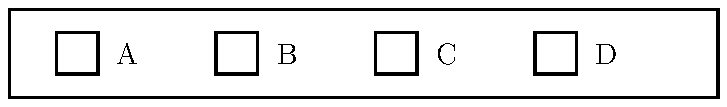
\includegraphics[width=0.85\textwidth]{choice4box}

\vspace{1cm}

\noindent\textbf{Question 2}

\vspace{0.3cm}
\noindent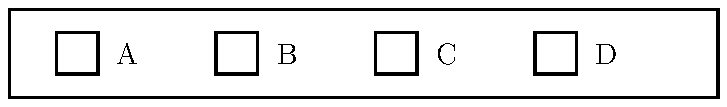
\includegraphics[width=0.85\textwidth]{choice4box}

\vspace{1cm}

\noindent\textbf{Question 3}

\vspace{0.3cm}
\noindent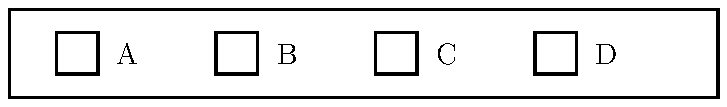
\includegraphics[width=0.85\textwidth]{choice4box}

% ------------------------------------------------------------------
% APPROACH 2 — Absolute positioning with TikZ overlay.
% Use this instead of approach 1 if you need precise (x, y) control.
% Coordinates are measured from the top-left of the page.
% Uncomment the block below to try it.
% ------------------------------------------------------------------

% \begin{tikzpicture}[remember picture, overlay]
%   % Place a choice4box at 3 cm from left, 10 cm from top
%   \node[anchor=north west] at
%     ([xshift=3cm, yshift=-10cm]current page.north west)
%     {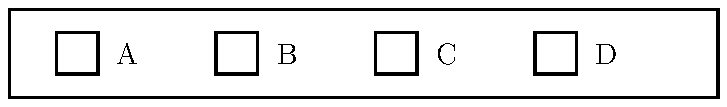
\includegraphics[width=0.85\textwidth]{choice4box}};
%
%   % Place another at 3 cm from left, 15 cm from top
%   \node[anchor=north west] at
%     ([xshift=3cm, yshift=-15cm]current page.north west)
%     {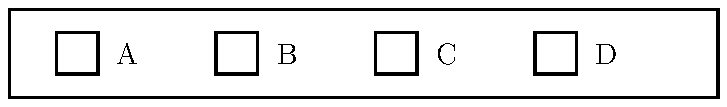
\includegraphics[width=0.85\textwidth]{choice4box}};
% \end{tikzpicture}

\end{document}
